% Journal draft. Neutral layout: move to the chosen journal's template once the journal is fixed.
% Rule (AGENTS.md §6, paper/README.md): every number comes from a file in experiments/, through generated macros and tables.
% Generated inputs: tables/rq2_*.tex, figs/rq2_stages.pdf <- scripts/rq2/rq2_report.py
%                   tables/c11x_explor.tex, tables/c11x_macros.tex <- scripts/c11x/export_explor.py
%                   tables/results_*.tex, figs/recall_iou.pdf <- scripts/c11x/export_results.py
% Red [TODO: ...] marks what is missing. Nothing marked TODO may be read as a finding.
\documentclass[11pt]{article}
\usepackage[margin=1in]{geometry}
\usepackage{amsmath,amssymb,booktabs,graphicx,xcolor,url}
\usepackage[hidelinks]{hyperref}
\newcommand{\todo}[1]{\textcolor{red}{[TODO: #1]}}
\newcommand{\rqNgt}{135{,}275}
\newcommand{\rqRescuedOne}{9{,}909}
\newcommand{\rqStarvedOne}{63}
\newcommand{\rqRescuedEight}{10{,}141}
\newcommand{\rqStarvedEight}{82}
\newcommand{\rqRescuedTwo}{10{,}663}
\newcommand{\rqStarvedTwo}{42}
\newcommand{\rqZeroCandVtA}{19.8}

\newcommand{\dAvtAtwo}{+0.0090}
\newcommand{\dAvtAtwoSceneLo}{+0.0052}
\newcommand{\dAvtAtwoSceneHi}{+0.0149}
\newcommand{\dAvtAtwoCombLo}{$-$0.0088}
\newcommand{\dAvtAtwoCombHi}{+0.0269}
\newcommand{\nCombExcl}{0}
\newcommand{\gateCoef}{$-$0.33}
\newcommand{\gateLo}{$-$0.50}
\newcommand{\gateHi}{$-$0.16}
\newcommand{\recallZero}{6.5\%}
\newcommand{\recallOne}{33.5\%}
\newcommand{\recallFive}{53.2\%}

\newcommand{\pOneSFour}{+0.0085}
\newcommand{\pOneSFive}{+0.0087}
\newcommand{\pOneMean}{+0.0086}
\newcommand{\pOneAzeroSFour}{0.0430}
\newcommand{\pOneAtwoSFour}{0.0515}
\newcommand{\pOneOldMin}{+0.0045}
\newcommand{\pOneOldMax}{+0.0155}
\newcommand{\pOneNmsSFour}{+0.0081}
\newcommand{\pOneNmsSFive}{+0.0081}
\newcommand{\apNewMean}{+0.0039}
\newcommand{\apsNewMean}{$-$0.0014}
\newcommand{\apmNewMean}{$-$0.0083}
\newcommand{\apsOldMean}{$-$0.0043}
\newcommand{\apmOldMean}{$-$0.0083}
\newcommand{\rzeroDap}{+0.0015}
\newcommand{\rzeroDval}{$-$0.019}
\newcommand{\valCOne}{+0.133}
\newcommand{\valCOneN}{947}
\newcommand{\valLocShare}{69.7}
\newcommand{\valMissShare}{29.0}
\newcommand{\mOneOld}{+0.068}
\newcommand{\mOneNew}{+0.067}
\newcommand{\mOneOldLow}{+0.135}
\newcommand{\mOneNewLow}{+0.136}
\newcommand{\mOneSeedMin}{+0.062}
\newcommand{\mOneSeedMax}{+0.078}
\newcommand{\vtDetAzero}{24.8}
\newcommand{\vtDetAtwo}{30.2}
\newcommand{\vtMissAzero}{47.4}
\newcommand{\vtMissAtwo}{41.9}
\newcommand{\vtLocAzero}{27.5}
\newcommand{\vtLocAtwo}{27.6}
\newcommand{\vtMissShareUndet}{60.0}
\newcommand{\vtLocShareUndetLow}{65.0}
\newcommand{\vtMissShareUndetLow}{33.4}
\newcommand{\vtDetAtwoLow}{45.3}
\newcommand{\vtLocAtwoLow}{35.5}
\newcommand{\vtMissAtwoLow}{18.2}
\newcommand{\starvedAzero}{5.8}
\newcommand{\starvedAtwo}{16.4}
\newcommand{\fedAzero}{30.4}
\newcommand{\fedAtwo}{34.3}
\newcommand{\recVtOne}{78.4}
\newcommand{\recVtHalf}{45.3}
\newcommand{\recVtThreeQ}{4.7}
\newcommand{\dropVt}{19.6}
\newcommand{\dropT}{13.5}
\newcommand{\recVtHalfAzeroHigh}{24.8}
\newcommand{\recVtHalfAtwoHigh}{30.2}
\newcommand{\tStarvedAzero}{15.0}
\newcommand{\tStarvedAtwo}{30.7}
\newcommand{\tStarvedN}{1{,}166}
\newcommand{\didLogit}{+0.98}
\newcommand{\vtZeroCandTest}{22.8}
\newcommand{\nVtTest}{44{,}177}
\newcommand{\nScenesTest}{8{,}107}
\newcommand{\nScenesVt}{3{,}492}
\newcommand{\aTwoOldSd}{0.0062}
\newcommand{\apmNeg}{5}
\newcommand{\apmSeeds}{5}
\newcommand{\aZeroOldMax}{0.0415}
\newcommand{\aZeroNewMin}{0.0430}
\newcommand{\pOneNewApMax}{+0.0063}


\begin{document}
\title{Candidate Floors for Tiny Oriented Objects:\\
A Stage-Wise Audit of Label Assignment in YOLO26n-OBB on AI-TOD-R}
\author{Vo Duc Nhat, Tran Loi Kieu Nhi, Tran Nguyen Minh Hai, Nguyen Tan Tai\\ FPT University, Vietnam
\todo{Confirm author order, name spelling (with or without diacritics), affiliations, emails and whether the mentor is a co-author.}}
\date{}
\maketitle

\begin{abstract}
One-stage detectors can give a tiny object no training signal when its box contains no anchor centre. Recent YOLO
releases enlarge tiny boxes during candidate selection to prevent this, a rule ablated on COCO with horizontal boxes in
single runs. We audit such candidate floors for oriented tiny objects with YOLO26n-OBB on the non-xView part of AI-TOD-R.
Tracing every ground-truth box through the assignment stages shows that without a floor \rqZeroCandVtA\% of very tiny
boxes ($<8$ px) have no candidate anchor, and that any floor removes this loss. On two training seeds that were not seen
when the comparison was fixed, the library's current floor raised AP$_{vt}$ by \pOneSFour{} and \pOneSFive{} over no
floor, matching three earlier exploratory seeds. A per-box analysis explains why the gain stays small: boxes that the floor
rescues gain more recall than other very tiny boxes, yet only \starvedAtwo\% of them are detected, and at a low score
threshold most undetected very tiny boxes have a prediction nearby that misses the IoU threshold. Once candidates are
restored, localisation appears to limit very tiny oriented objects in this setting more than assignment does.
\end{abstract}

\section{Introduction}
Aerial benchmarks contain objects far smaller than the coarsest assumptions of general detectors. In AI-TOD-R the mean
object size is about 10.6 px \cite{aitodr}, close to the finest stride of a typical feature pyramid. Under task-aligned
assignment \cite{tood}, an anchor can become a positive only if its centre lies inside the box, so a very small box can
receive no positive at all. YOLO26 \cite{yolo26} introduces Small-Target-Aware Label Assignment (STAL): sides below a
threshold are replaced by a larger value during candidate selection only, while scoring, target assignment and
regression keep the original box.

Three gaps motivate this audit. First, the published ablation of STAL uses COCO with horizontal boxes and reports single
values without repeated runs \cite[Table 6]{yolo26}; its oriented-box section does not evaluate the rule. Second, the rule
applied to oriented boxes has changed across library releases \cite{ultralytics}: no floor up to release 8.4.7; sides below
8 px replaced by 16 px from 8.4.8 (applied in place until a fix in 8.4.39); and sides below 16 px replaced by 16 px from
8.4.128 on.\footnote{From the history of \texttt{ultralytics/utils/tal.py}, release tags checked on 8 October 2026.}
Results for ``STAL'' therefore depend on the package version. Third, tiny-object work reports that small objects receive
fewer positives \cite{aitodr}, and several assigners give them more \cite{cdcedet,dala,ngla}, but in the work we read we found no
per-box account of where they lose positives under a deployed rule, nor of what happens to a box after it is given
candidates.

We ask: (Q1) at which assignment stage do tiny oriented boxes lose supervision, under each floor? (Q2) does a floor raise
AP$_{vt}$ on two seeds that were not seen when the comparison was chosen? (Q3) if a floor gives almost every box a
candidate, why does AP$_{vt}$ stay low: are the rescued boxes missed, poorly localised, or taken by neighbours?

Our contributions are: an exact label-only decomposition of the candidate stage, validated against the library code; a
preregistered comparison extended with two new seeds, reported with scene and seed uncertainty; and a per-box error
analysis linking assignment geometry to detection outcome, which points to localisation as the remaining limit. This is
an audit of an existing rule, not a new detector.

\section{Related Work}
\textbf{Label assignment for tiny objects.} RFLA \cite{rfla} and NWD-based assignment \cite{aitodv2} replace IoU-based
matching with measures less sensitive to small offsets. DCFL \cite{aitodr} assigns oriented tiny objects dynamically and
sets the benchmark for AI-TOD-R; that paper notes qualitatively that tiny objects receive fewer positives, and its
benchmark table has no YOLO-family row. Recent methods enlarge or re-rank the positive set of tiny objects: NGLA
\cite{ngla} measures similarity between Gaussian box models and ranks candidates by classification and localisation
quality (horizontal boxes, AI-TOD-v2 and VisDrone, MMDetection detectors); DALA \cite{dala} sets the number of positives
per object adaptively; MFN-Net \cite{mfnnet} combines flexible label assignment with multi-scale fusion on SODA-A and
AI-TOD. Closest to our data, CDCEDet \cite{cdcedet} generates scale-adaptive anchors and adaptive IoU thresholds to give
tiny objects more positives, together with frequency-domain feature fusion, and reports gains on AI-TOD-v2 and AI-TOD-R.
These works propose new assigners and show that more positives help; we instead measure, box by box, where a deployed
real-time rule loses positives and what happens to boxes after they are given candidates. \todo{Full texts of DALA,
MFN-Net and CDCEDet not yet read (abstract or publisher summary only); NGLA read by section structure and keyword search.
Check that none of them reports a per-box stage or error analysis of the kind in Section~\ref{sec:link}.}

\textbf{Floors and pseudo-boxes.} STAL \cite{yolo26} is ablated with reference sizes 8, 16 and 32 on COCO. OSCAR
\cite{oscar} sweeps square pseudo-boxes for sub-stride infrared targets with horizontal boxes and reports a non-monotonic
optimum, so ``floor size matters'' is known. We study the oriented, multi-level, dense case.

\textbf{Oriented assignment.} EARL \cite{earl}, SARFA-Net \cite{sarfa} and ARA \cite{ara} make assignment for oriented boxes
shape- or aspect-ratio-aware, on general aerial benchmarks rather than tiny-object ones. MCSA \cite{mcsa} targets oriented
tiny objects with a multi-factor sample assignment on a RetinaNet-OBB baseline, evaluated on DOTA and DIOR-R; it does not use
AI-TOD-R or a YOLO detector. \todo{ARA read at abstract level only.}

\textbf{YOLO-OBB on AI-TOD.} DIA-YOLO \cite{diayolo} reports a YOLOv11-OBB baseline and a depth-fusion backbone on 18,730
AI-TOD images. It changes the network input and backbone, and we found no treatment of label assignment in its method and
results sections. Its protocol differs from ours, so our numbers are not comparable with it.

\textbf{Error analysis.} TIDE \cite{tide} attributes detection errors to types. We use a simpler box-centred variant with
rotated IoU and do not estimate its $\Delta$AP.

\section{Assignment Stages and Candidate Floors}
YOLO26-OBB places anchor centres at $((i+\tfrac12)s,(j+\tfrac12)s)$ for $s\in\{8,16,32\}$. Training uses the task-aligned
assigner \cite{tood} with ProbIoU \cite{probiou}: (1) an anchor is a \emph{candidate} of a box if it lies inside the box's
candidate region; (2) the top-$k$ candidates by alignment metric are kept ($k=10$ one-to-many; $k=7$ then $k_2=1$
one-to-one); (3) an anchor kept by several boxes goes to the box of highest predicted overlap. A floor rule replaces each
side $<\tau$ by $f$ in step (1) only: A0 none; A1 $\tau=8, f=16$; A8 $\tau=f=8\sqrt2$; A2 $\tau=f=16$ (the current library
rule).

A region whose short side is at least $\sqrt2\,s$ contains an anchor of stride $s$ for every position and angle. This
guarantees a candidate. It does not guarantee a positive, useful supervision or an AP optimum.

\textbf{Label-only stage analysis.} Step (1) is exact: our implementation reproduces the library's candidate mask on random
boxes (unit test). Steps (2)--(3) need predictions, so we replace the alignment metric by anchor-to-centre distance and
report the result as a \emph{proxy}, together with the exact count of boxes with no candidate, which is a lower bound on
boxes without a positive. With no mosaic, scaling or translation and $800\times800$ inputs, flips map the lattice onto
itself, so the counts hold for every training sample.

\section{Experimental Setup}
\textbf{Data.} AI-TOD-R \cite{aitodr}, non-xView protocol (woX): 8,426 train, 936 val and 9,261 test images, with the val
split made by scene. Results are not comparable with the full-benchmark Table II of \cite{aitodr}.

\textbf{Training.} YOLO26n-OBB \cite{yolo26} from COCO weights, Ultralytics 8.4.174 pinned, 24 epochs, SGD, imgsz 800, flips
only, batch 16, on one A100 GPU. The benchmark of \cite{aitodr} uses 12 and 40 epochs; val AP was still rising at epoch 24, so
conclusions hold for this recipe only. New seeds use the same training code as the exploratory ones.

\textbf{Evaluation.} Official AITODReval (1,500 detections per image and class, \texttt{max\_det}=12,000; oracle AP 0.996),
scoring \texttt{last.pt}, with the end-to-end (e2e) and NMS heads reported separately.

\textbf{Sequence of the study.} (i) Twelve exploratory runs (A0, A1, A8, A2 $\times$ seeds 1--3) on the test set. (ii) A
val-only per-box analysis of the same twelve runs, with a stopping rule written before it was run, which decided whether
new seeds were worth training and which arms to keep. (iii) A preregistration annex fixed before training, merged on
6 November 2026 (repository commit \texttt{d8b9d99}). (iv) Training of A0 and A2 on seeds 4 and 5, plus a reproducibility
run R0 that repeats A2 seed 1.

\textbf{Primary comparison.} P1 is $\Delta$AP$_{vt}$(A2$-$A0) with the e2e head. The pair and the metric were chosen after
seeing seeds 1--3, so P1 is judged on the two new seeds only: it counts as replicated if $\Delta>0$ on both and their mean
is at least 0.006, the minimal effect of interest derived from seed variation. This is a replication on two new seeds, not
an independent confirmation, and a decision rule rather than a statistical test. Seeds 1--3 and 4--5 are pooled only if
R0 reproduces the earlier run (Section~\ref{sec:acc}).

\textbf{Per-box analysis.} On test boxes, a box is detected if a same-class prediction with score $\geq 0.25$ matches it at
rotated IoU $\geq 0.5$ under greedy score-ordered matching; score $\geq 0.05$ is a sensitivity check. Undetected boxes get
one fate, in this order: taken by a neighbour's prediction (a same-class prediction reaches IoU 0.5 but is matched to
another box), wrong class, poor localisation (best same-class IoU in $[0.1, 0.5)$), both, or missed (no prediction reaches
IoU 0.1). M1 is a difference in differences of recall: [A2$-$A0] on very tiny boxes that A0 leaves without a candidate,
minus the same on other very tiny boxes. Its uncertainty combines a scene-clustered bootstrap ($B=10{,}000$) with seed
variation, $\Delta\pm t_{0.975,n-1}\sqrt{\mathrm{se}_\text{scene}^2+\mathrm{se}_\text{seed}^2}$.

\section{Results}
\subsection{Where boxes lose candidates and positives (labels only)}
Table~\ref{tab:stages} and Fig.~\ref{fig:stages} use all \rqNgt{} boxes of woX train+val. Relative to A0, A2 rescues
\rqRescuedTwo{} boxes from zero positives (proxy) and newly starves \rqStarvedTwo{}; A8: \rqRescuedEight{} and
\rqStarvedEight{}; A1: \rqRescuedOne{} and \rqStarvedOne{}. Table~\ref{tab:density} shows that the remaining loss under a floor
sits in dense clusters. These are predictions from geometry; Section~\ref{sec:link} tests them on detector output.

\begin{table}[t]\centering\caption{Assignment stages per box, woX train+val (labels only).}
\label{tab:stages}\footnotesize\begin{tabular}{lrrrr}
\toprule
 & A0 & A1 & A8 & A2 \\
\midrule
\multicolumn{5}{l}{\textit{very tiny ($<$8 px)}{,} $n=50{,}263$} \\
\quad candidates / GT & 1.04 & 3.79 & 2.61 & 5.37 \\
\quad zero candidates (\%) & 19.8 & 0.0 & 0.0 & 0.0 \\
\quad shared candidates (\%) & 5.1 & 44.9 & 34.5 & 50.6 \\
\quad zero positives, proxy (\%) & 20.7 & 2.7 & 2.4 & 1.4 \\
\multicolumn{5}{l}{\textit{tiny (8--16 px)}{,} $n=66{,}414$} \\
\quad candidates / GT & 2.92 & 4.18 & 3.82 & 5.98 \\
\quad zero candidates (\%) & 1.2 & 0.0 & 0.0 & 0.0 \\
\quad shared candidates (\%) & 7.3 & 18.3 & 13.8 & 27.5 \\
\quad zero positives, proxy (\%) & 1.5 & 0.3 & 0.2 & 0.1 \\
\multicolumn{5}{l}{\textit{small (16--32 px)}{,} $n=14{,}877$} \\
\quad candidates / GT & 10.31 & 10.34 & 10.42 & 11.43 \\
\quad zero candidates (\%) & 0.0 & 0.0 & 0.0 & 0.0 \\
\quad shared candidates (\%) & 9.3 & 9.8 & 9.7 & 13.1 \\
\quad zero positives, proxy (\%) & 0.0 & 0.0 & 0.0 & 0.0 \\
\bottomrule
\end{tabular}
\end{table}
\begin{table}[t]\centering\caption{Boxes without any positive (proxy, \%) by number of box centres within 16 px.}
\label{tab:density}\footnotesize\begin{tabular}{llrrrrr}
\toprule
size & neighbours & $n$ & A0 & A1 & A8 & A2 \\
\midrule
very tiny & isolated & 13{,}765 & 18.2 & 0.0 & 0.0 & 0.0 \\
very tiny & 1--2 & 16{,}750 & 19.0 & 0.3 & 0.4 & 0.1 \\
very tiny & $\geq$3 & 19{,}748 & 23.9 & 6.7 & 5.7 & 3.4 \\
tiny & isolated & 31{,}841 & 1.0 & 0.0 & 0.0 & 0.0 \\
tiny & 1--2 & 27{,}898 & 1.4 & 0.1 & 0.1 & 0.1 \\
tiny & $\geq$3 & 6{,}675 & 4.3 & 2.1 & 1.9 & 1.2 \\
\bottomrule
\end{tabular}
\end{table}
\begin{figure}[t]\centering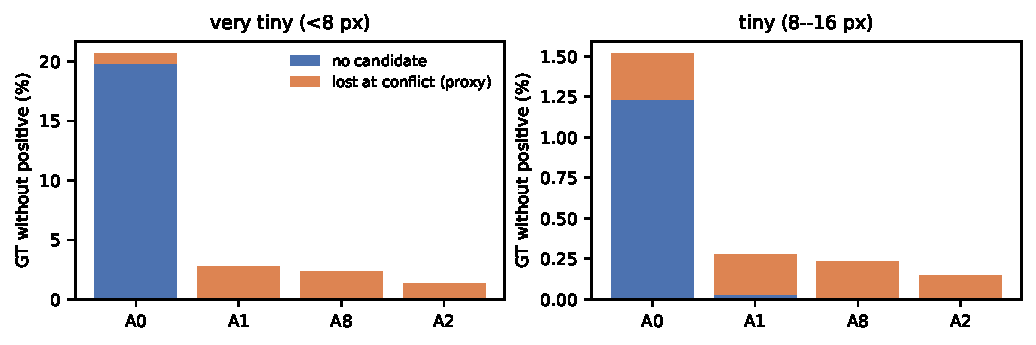
\includegraphics[width=0.7\columnwidth]{figs/rq2_stages}
\caption{Share of boxes without a positive: no candidate (exact) and lost at conflict (proxy).}
\label{fig:stages}\end{figure}

\subsection{Detection accuracy}\label{sec:acc}
\textbf{Exploratory, seeds 1--3 (Table~\ref{tab:explor}).} For A2$-$A0 with the e2e head, $\Delta$AP$_{vt}$ is \dAvtAtwo{}. The
scene-only interval is [\dAvtAtwoSceneLo{}, \dAvtAtwoSceneHi{}], while the interval that also includes seed variation is
[\dAvtAtwoCombLo{}, \dAvtAtwoCombHi{}]. Of the 40 combined intervals, \nCombExcl{} exclude zero. With three seeds these
results do not support a claim in either direction. The preregistered test of candidate count on val did not support a
positive effect (coefficient \gateCoef{}, 95\% CI [\gateLo{}, \gateHi{}]), so a planned adaptive floor was dropped.

\textbf{Val check before training.} On val, very tiny boxes that A0 leaves without a candidate gained \valCOne{} recall under
A2 (\valCOneN{} boxes, mean over seeds 1--3), and among very tiny boxes that A2 still missed at score $\geq 0.05$,
\valLocShare\% were poorly localised and \valMissShare\% had no prediction nearby. The rule therefore called for training.
The density contrast between A2 and A8 changed sign across seeds, so A8 was dropped from the new runs. A8 had the highest
very-tiny recall of the four arms on val; the rule asked about the density contrast, not about which arm is best, and we did
not test A8 further.

\textbf{P1, seeds 4--5 (Table~\ref{tab:p1}).} $\Delta$AP$_{vt}$(A2$-$A0) was \pOneSFour{} on seed 4 and \pOneSFive{} on seed 5,
mean \pOneMean{}: P1 is replicated under the preregistered rule. Both values lie within the range of the exploratory seeds
(\pOneOldMin{} to \pOneOldMax{}). With the NMS head the differences were \pOneNmsSFour{} and \pOneNmsSFive{}. Overall AP rose
by \apNewMean{} on average over seeds 4--5, and AP$_m$ fell by \apmNewMean{} in both seed groups; AP$_s$ changed by
\apsNewMean{} on seeds 4--5 and \apsOldMean{} on seeds 1--3, with mixed signs across seeds. These are descriptive.

\textbf{Reproducibility check.} R0 repeated A2 seed 1: test AP differed by \rzeroDap{}, within the preset 0.005, but val
mAP at epoch 24 differed by \rzeroDval{}, outside it. Following the annex, seeds 1--3 and 4--5 are reported apart and never
pooled. The cause of the val difference is not known; the training environment showed a different numpy version.

\begin{table}[t]\centering\caption{Test AP per seed, e2e head, woX. $\Delta$ is A2 minus A0. Seeds 1--3 were seen before P1 was
fixed; seeds 4--5 were not. The groups are not pooled because R0 did not reproduce.}\label{tab:p1}\scriptsize
\begin{tabular}{llrrrrrrr}
\toprule
Seeds & Seed & AP$_{vt}$ A0 & AP$_{vt}$ A2 & $\Delta$AP$_{vt}$ & $\Delta$AP$_t$ & $\Delta$AP$_s$ & $\Delta$AP$_m$ & $\Delta$AP \\
\midrule
1--3, exploratory & 1 & 0.0411 & 0.0456 & +0.0045 & +0.0071 & $-$0.0112 & $-$0.0074 & +0.0009 \\
 & 2 & 0.0415 & 0.0570 & +0.0155 & +0.0074 & +0.0109 & $-$0.0042 & +0.0083 \\
 & 3 & 0.0401 & 0.0472 & +0.0070 & +0.0042 & $-$0.0125 & $-$0.0132 & +0.0014 \\
 & mean & & & +0.0090 & +0.0062 & $-$0.0043 & $-$0.0083 & +0.0035 \\
\midrule
4--5, new & 4 & 0.0430 & 0.0515 & +0.0085 & +0.0077 & $-$0.0009 & $-$0.0028 & +0.0063 \\
 & 5 & 0.0430 & 0.0518 & +0.0087 & +0.0048 & $-$0.0018 & $-$0.0138 & +0.0014 \\
 & mean & & & +0.0086 & +0.0063 & $-$0.0014 & $-$0.0083 & +0.0039 \\
\bottomrule
\end{tabular}
\end{table}

\begin{table}[t]\centering\caption{Exploratory $\Delta$ on seeds 1--3, woX test. Scene: scene-clustered bootstrap only. Scene + seed:
combined interval with $t$ on 2 degrees of freedom.}\label{tab:explor}\scriptsize\begin{tabular}{llrcc}
\toprule
Head & Pair and metric & $\Delta$ & Scene 95\% CI & Scene + seed 95\% CI \\
\midrule
e2e & A1$-$A0, AP$_{vt}$ & +0.0074 & [+0.0032, +0.0158] & [$-$0.0094, +0.0243] \\
e2e & A1$-$A0, AP$_{t}$ & +0.0016 & [$-$0.0006, +0.0032] & [$-$0.0056, +0.0088] \\
e2e & A1$-$A0, AP$_{s}$ & $-$0.0064 & [$-$0.0102, $-$0.0034] & [$-$0.0200, +0.0073] \\
e2e & A1$-$A0, AP$_{m}$ & $-$0.0022 & [$-$0.0089, +0.0058] & [$-$0.0227, +0.0182] \\
e2e & A1$-$A0, AP & +0.0006 & [$-$0.0009, +0.0024] & [$-$0.0074, +0.0087] \\
e2e & A8$-$A0, AP$_{vt}$ & +0.0071 & [+0.0000, +0.0115] & [$-$0.0089, +0.0230] \\
e2e & A8$-$A0, AP$_{t}$ & +0.0042 & [+0.0006, +0.0073] & [$-$0.0082, +0.0167] \\
e2e & A8$-$A0, AP$_{s}$ & $-$0.0026 & [$-$0.0068, +0.0005] & [$-$0.0180, +0.0127] \\
e2e & A8$-$A0, AP$_{m}$ & $-$0.0029 & [$-$0.0086, +0.0044] & [$-$0.0321, +0.0263] \\
e2e & A8$-$A0, AP & +0.0025 & [+0.0005, +0.0047] & [$-$0.0105, +0.0155] \\
e2e & A2$-$A0, AP$_{vt}$ & +0.0090 & [+0.0052, +0.0149] & [$-$0.0088, +0.0269] \\
e2e & A2$-$A0, AP$_{t}$ & +0.0062 & [+0.0041, +0.0082] & [$-$0.0001, +0.0126] \\
e2e & A2$-$A0, AP$_{s}$ & $-$0.0043 & [$-$0.0088, $-$0.0003] & [$-$0.0383, +0.0297] \\
e2e & A2$-$A0, AP$_{m}$ & $-$0.0083 & [$-$0.0168, $-$0.0010] & [$-$0.0290, +0.0125] \\
e2e & A2$-$A0, AP & +0.0035 & [+0.0017, +0.0056] & [$-$0.0076, +0.0147] \\
e2e & A2$-$A8, AP$_{vt}$ & +0.0019 & [$-$0.0033, +0.0118] & [$-$0.0228, +0.0267] \\
e2e & A2$-$A8, AP$_{t}$ & +0.0020 & [$-$0.0010, +0.0055] & [$-$0.0141, +0.0181] \\
e2e & A2$-$A8, AP$_{s}$ & $-$0.0016 & [$-$0.0049, +0.0021] & [$-$0.0389, +0.0357] \\
e2e & A2$-$A8, AP$_{m}$ & $-$0.0054 & [$-$0.0139, +0.0006] & [$-$0.0449, +0.0341] \\
e2e & A2$-$A8, AP & +0.0011 & [$-$0.0010, +0.0032] & [$-$0.0180, +0.0201] \\
\midrule
nms & A1$-$A0, AP$_{vt}$ & +0.0065 & [+0.0034, +0.0127] & [$-$0.0124, +0.0255] \\
nms & A1$-$A0, AP$_{t}$ & +0.0013 & [$-$0.0014, +0.0033] & [$-$0.0097, +0.0122] \\
nms & A1$-$A0, AP$_{s}$ & $-$0.0066 & [$-$0.0106, $-$0.0031] & [$-$0.0311, +0.0178] \\
nms & A1$-$A0, AP$_{m}$ & $-$0.0069 & [$-$0.0143, +0.0022] & [$-$0.0252, +0.0113] \\
nms & A1$-$A0, AP & +0.0002 & [$-$0.0018, +0.0020] & [$-$0.0086, +0.0089] \\
nms & A8$-$A0, AP$_{vt}$ & +0.0057 & [$-$0.0004, +0.0089] & [$-$0.0074, +0.0188] \\
nms & A8$-$A0, AP$_{t}$ & +0.0037 & [$-$0.0002, +0.0067] & [$-$0.0094, +0.0167] \\
nms & A8$-$A0, AP$_{s}$ & $-$0.0045 & [$-$0.0083, $-$0.0013] & [$-$0.0180, +0.0089] \\
nms & A8$-$A0, AP$_{m}$ & $-$0.0087 & [$-$0.0151, $-$0.0014] & [$-$0.0293, +0.0120] \\
nms & A8$-$A0, AP & +0.0015 & [$-$0.0006, +0.0037] & [$-$0.0104, +0.0134] \\
nms & A2$-$A0, AP$_{vt}$ & +0.0071 & [+0.0028, +0.0150] & [$-$0.0083, +0.0224] \\
nms & A2$-$A0, AP$_{t}$ & +0.0047 & [+0.0018, +0.0070] & [$-$0.0020, +0.0113] \\
nms & A2$-$A0, AP$_{s}$ & $-$0.0095 & [$-$0.0133, $-$0.0049] & [$-$0.0340, +0.0150] \\
nms & A2$-$A0, AP$_{m}$ & $-$0.0102 & [$-$0.0196, $-$0.0011] & [$-$0.0347, +0.0143] \\
nms & A2$-$A0, AP & +0.0010 & [$-$0.0012, +0.0033] & [$-$0.0070, +0.0090] \\
nms & A2$-$A8, AP$_{vt}$ & +0.0013 & [$-$0.0039, +0.0121] & [$-$0.0182, +0.0209] \\
nms & A2$-$A8, AP$_{t}$ & +0.0010 & [$-$0.0013, +0.0036] & [$-$0.0084, +0.0104] \\
nms & A2$-$A8, AP$_{s}$ & $-$0.0050 & [$-$0.0079, $-$0.0009] & [$-$0.0263, +0.0164] \\
nms & A2$-$A8, AP$_{m}$ & $-$0.0015 & [$-$0.0092, +0.0054] & [$-$0.0331, +0.0300] \\
nms & A2$-$A8, AP & $-$0.0005 & [$-$0.0023, +0.0013] & [$-$0.0118, +0.0108] \\
\bottomrule
\end{tabular}
\end{table}

\subsection{What happens to boxes after assignment}\label{sec:link}
\textbf{Rescued boxes (M1, Table~\ref{tab:m1}).} Very tiny boxes that A0 leaves without a candidate gained more recall under A2
than other very tiny boxes: \mOneOld{} on seeds 1--3 and \mOneNew{} on seeds 4--5 at score $\geq 0.25$, and \mOneOldLow{} and
\mOneNewLow{} at score $\geq 0.05$. All five per-seed values at score $\geq 0.25$ were positive (\mOneSeedMin{} to
\mOneSeedMax{}). With only two seeds, the combined interval of seeds 4--5 contains zero because the $t$ factor on one degree of
freedom is 12.7, not because the sign changed. M1 had already been seen on val, so on test it is a check on new images
and seeds rather than an unseen prediction. A difference in differences does not remove every other difference between the
two groups of boxes, such as size within the very tiny bin.

Even so, rescue does not mean detection. Under A2, \starvedAtwo\% of the boxes that A0 starves were detected at score
$\geq 0.25$, against \starvedAzero\% under A0 and \fedAtwo\% for the other very tiny boxes under A2 (\fedAzero\% under A0).
That A0 detects some boxes without any candidate shows that neighbouring anchors' predictions can still cover them.

\textbf{Fate of very tiny boxes (Table~\ref{tab:fates}, Fig.~\ref{fig:iou}).} At score $\geq 0.25$, A2 detected \vtDetAtwo\% of
very tiny boxes against \vtDetAzero\% for A0; the gain came from fewer missed boxes (\vtMissAtwo\% against \vtMissAzero\%),
while poorly localised boxes stayed at about the same share (\vtLocAtwo\% and \vtLocAzero\%). Taken by a neighbour and wrong
class were rare for every arm. Missed was the largest fate among undetected very tiny boxes at score $\geq 0.25$
(\vtMissShareUndet\%), as predicted, but at score $\geq 0.05$ poor localisation became the largest (\vtLocShareUndetLow\% against
\vtMissShareUndetLow\%). Part of what counts as missed at the higher threshold is therefore a box in roughly the right place
with a low score.

Recall depends strongly on the IoU threshold for very tiny boxes. Under A2 at score $\geq 0.05$, \recVtOne\% of them had a
same-class prediction at IoU $\geq 0.1$, \recVtHalf\% at 0.5 and \recVtThreeQ\% at 0.75. The drop from IoU 0.25 to 0.5 was
\dropVt{} points for very tiny boxes and \dropT{} points for tiny ones (score $\geq 0.25$), as predicted. The fate and IoU tables
average seeds 1--5; per-seed versions are not in the repository, and their spread across seeds is small.

\begin{table}[t]\centering\caption{M1: difference in differences of recall, A2$-$A0, very tiny boxes that A0 starves minus other very
tiny boxes, e2e head, woX test.}\label{tab:m1}\footnotesize\begin{tabular}{llrcc}
\toprule
Score & Seeds & DiD & Scene 95\% CI & Scene + seed 95\% CI \\
\midrule
$\geq 0.25$ & 1--3 & +0.068 & [+0.055, +0.080] & [+0.033, +0.103] \\
 & 4--5 & +0.067 & [+0.054, +0.078] & [$-$0.023, +0.157] \\
$\geq 0.05$ & 1--3 & +0.135 & [+0.116, +0.152] & [+0.093, +0.177] \\
 & 4--5 & +0.136 & [+0.118, +0.154] & [$-$0.004, +0.277] \\
\bottomrule
\end{tabular}
\end{table}
\begin{table}[t]\centering\caption{Fate of boxes, \% of boxes in the size bin, e2e head, mean over seeds 1--5.}\label{tab:fates}
\scriptsize\begin{tabular}{lllrrrrrr}
\toprule
Score & Size & Arm & detected & neighbour & class & localisation & both & missed \\
\midrule
$\geq 0.25$ & very tiny & A0 & 24.8 & 0.0 & 0.1 & 27.5 & 0.3 & 47.4 \\
 &  & A2 & 30.2 & 0.0 & 0.1 & 27.6 & 0.3 & 41.9 \\
 & tiny & A0 & 53.9 & 0.2 & 0.2 & 18.9 & 0.2 & 26.6 \\
 &  & A2 & 57.0 & 0.2 & 0.2 & 18.7 & 0.2 & 23.8 \\
\midrule
$\geq 0.05$ & very tiny & A0 & 39.2 & 0.0 & 0.2 & 39.3 & 0.8 & 20.6 \\
 &  & A2 & 45.3 & 0.0 & 0.2 & 35.5 & 0.7 & 18.2 \\
 & tiny & A0 & 68.1 & 0.1 & 0.3 & 20.6 & 0.4 & 10.4 \\
 &  & A2 & 69.3 & 0.1 & 0.3 & 19.8 & 0.4 & 10.1 \\
\bottomrule
\end{tabular}
\end{table}
\begin{figure}[t]\centering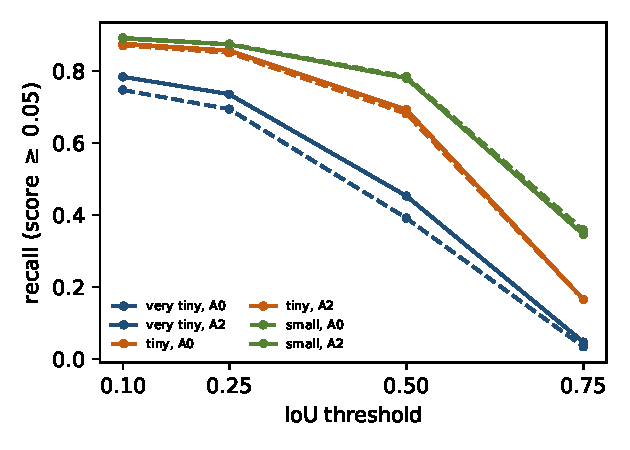
\includegraphics[width=0.6\columnwidth]{figs/recall_iou}
\caption{Recall against the IoU threshold, score $\geq 0.05$, e2e head, mean over seeds 1--5.}\label{fig:iou}\end{figure}

\section{Discussion}
\textbf{The floor works where it is meant to, and that is not enough.} Without a floor about one very tiny box in five has no
candidate. The library's floor removes this, and on two new seeds AP$_{vt}$ rose by about the same amount as on the
exploratory seeds. The boxes that the floor rescues gain the most recall, which is consistent with the mechanism the rule
targets. Since A2 also changes the candidate region of nearly every other box, the gain is not explained by rescue alone.

\textbf{Localisation is the remaining limit.} When low-scoring predictions are kept (score $\geq 0.05$), most very tiny boxes
that the detector does not count as found have a prediction of the right class nearby whose overlap falls short of the IoU
threshold, and recall falls steeply between IoU 0.25 and 0.5. At score $\geq 0.25$ more of them are simply missed, so low
confidence on these boxes is part of the same problem. A
shift of one or two pixels is a large fraction of a box under 8 px, so IoU-based matching is harsh at this size; this agrees
with the motivation of distance-based measures for tiny objects \cite{aitodv2}. In this setting, a better candidate rule can
only move boxes from missed to found if the predicted box is accurate enough to count. We expect larger gains from improving
localisation of very tiny oriented boxes, or from evaluation that is less sensitive to small offsets, than from further
changes to candidate selection. This is a hypothesis for future work, not a result of this study.

\textbf{Cost.} AP$_m$ fell in both seed groups, while overall AP rose slightly. A floor of 16 px enlarges the candidate region
of every box below that size, which can pull anchors away from larger neighbours; we did not test this mechanism.

\textbf{Which floor.} We kept the library default, A2, as the primary arm. A8, the smallest floor that guarantees a candidate,
had the highest recall on val but was not trained on new seeds. Whether the coverage-minimal floor matches or beats the
default remains open.

\textbf{Limitations.} One detector size (YOLO26n); a 24-epoch recipe; the non-xView subset of one dataset, with no second
dataset run; a proxy for assignment stages 2--3; P1 was chosen after the exploratory seeds and is judged on two new
seeds by a decision rule, not a test; the reproducibility check failed on val, so seeds 1--5 are not pooled; per-box tables
average seeds 1--5; box-level fates use one greedy matching and fixed thresholds; label noise matters at a few pixels, as the
evaluator's round trip already shows (only part of the boxes reach IoU $\geq 0.999$ with themselves). During the study, NMS
result files of eight exploratory runs were lost from shared storage and rebuilt from the original evaluation cache; this
affects only NMS-head tables, and the rebuilt values match those recorded before the loss.

\section{Conclusion}
For very tiny oriented objects in AI-TOD-R, YOLO26n-OBB without a candidate floor leaves about one box in five with no
candidate anchor. The library's current floor removes this loss and raised AP$_{vt}$ on two new seeds by an amount close to
the exploratory estimate. Boxes rescued by the floor gain the most recall, yet most very tiny boxes still go uncounted, and
among those with a low-scoring prediction kept, the predicted box is usually close but not accurate enough to pass the IoU
threshold. Once candidates are restored, localisation and confidence on very tiny boxes, rather than assignment, are the
limits to address.

\section*{Reproducibility}
Preregistration, analysis code, notebooks and result files: \url{https://github.com/VoDucNhatku/nckh-group7-tiny-obb}
(\texttt{experiments/}, \texttt{scripts/rq2/}, \texttt{scripts/c11x/}). Training and evaluation code \texttt{scripts/c11/}:
\todo{publish}. Model weights and DOTA-format predictions: \todo{release link}.

\bibliographystyle{unsrt}
\bibliography{refs}
\end{document}
